\appendix
\chapter{Art�culos}

\section{Aplicaciones}
\subsection{En Hardware Evolutivo}
Las plataformas desarrolladas en este trabajo fueron utilizadas como una forma novedosa y econ�mica de implementar algoritmos de hardware evolutivo, la posibilidad de tener una FPGA y un procesador en la misma placa permiti� la implementaci�n de algoritmos gen�ticos de forma intr�nseca, es decir, verificando el nivel de ajuste de cada individuo a la soluci�n requerida dentro del mismo dispositivo. En esta �rea se generaron dos art�culos:

\textbf{Intrinsic Evolvable Hardware for Combinatorial Synthesis Based on SoC+FPGA and GPU Platforms} Ser� publicado en la conferencia \textit{Genetic and Evolutionary Computation Conference} GECCO 2011; clasificada 7ma entre 711 conferencias en inteligencia artificial (AI conference ranking) y es pubicado por ACM (Association for Computing Machinery \footnote{ACM, es la sociedad educativa y cient�fica  inform�tica m�s grande del mundo.}) 


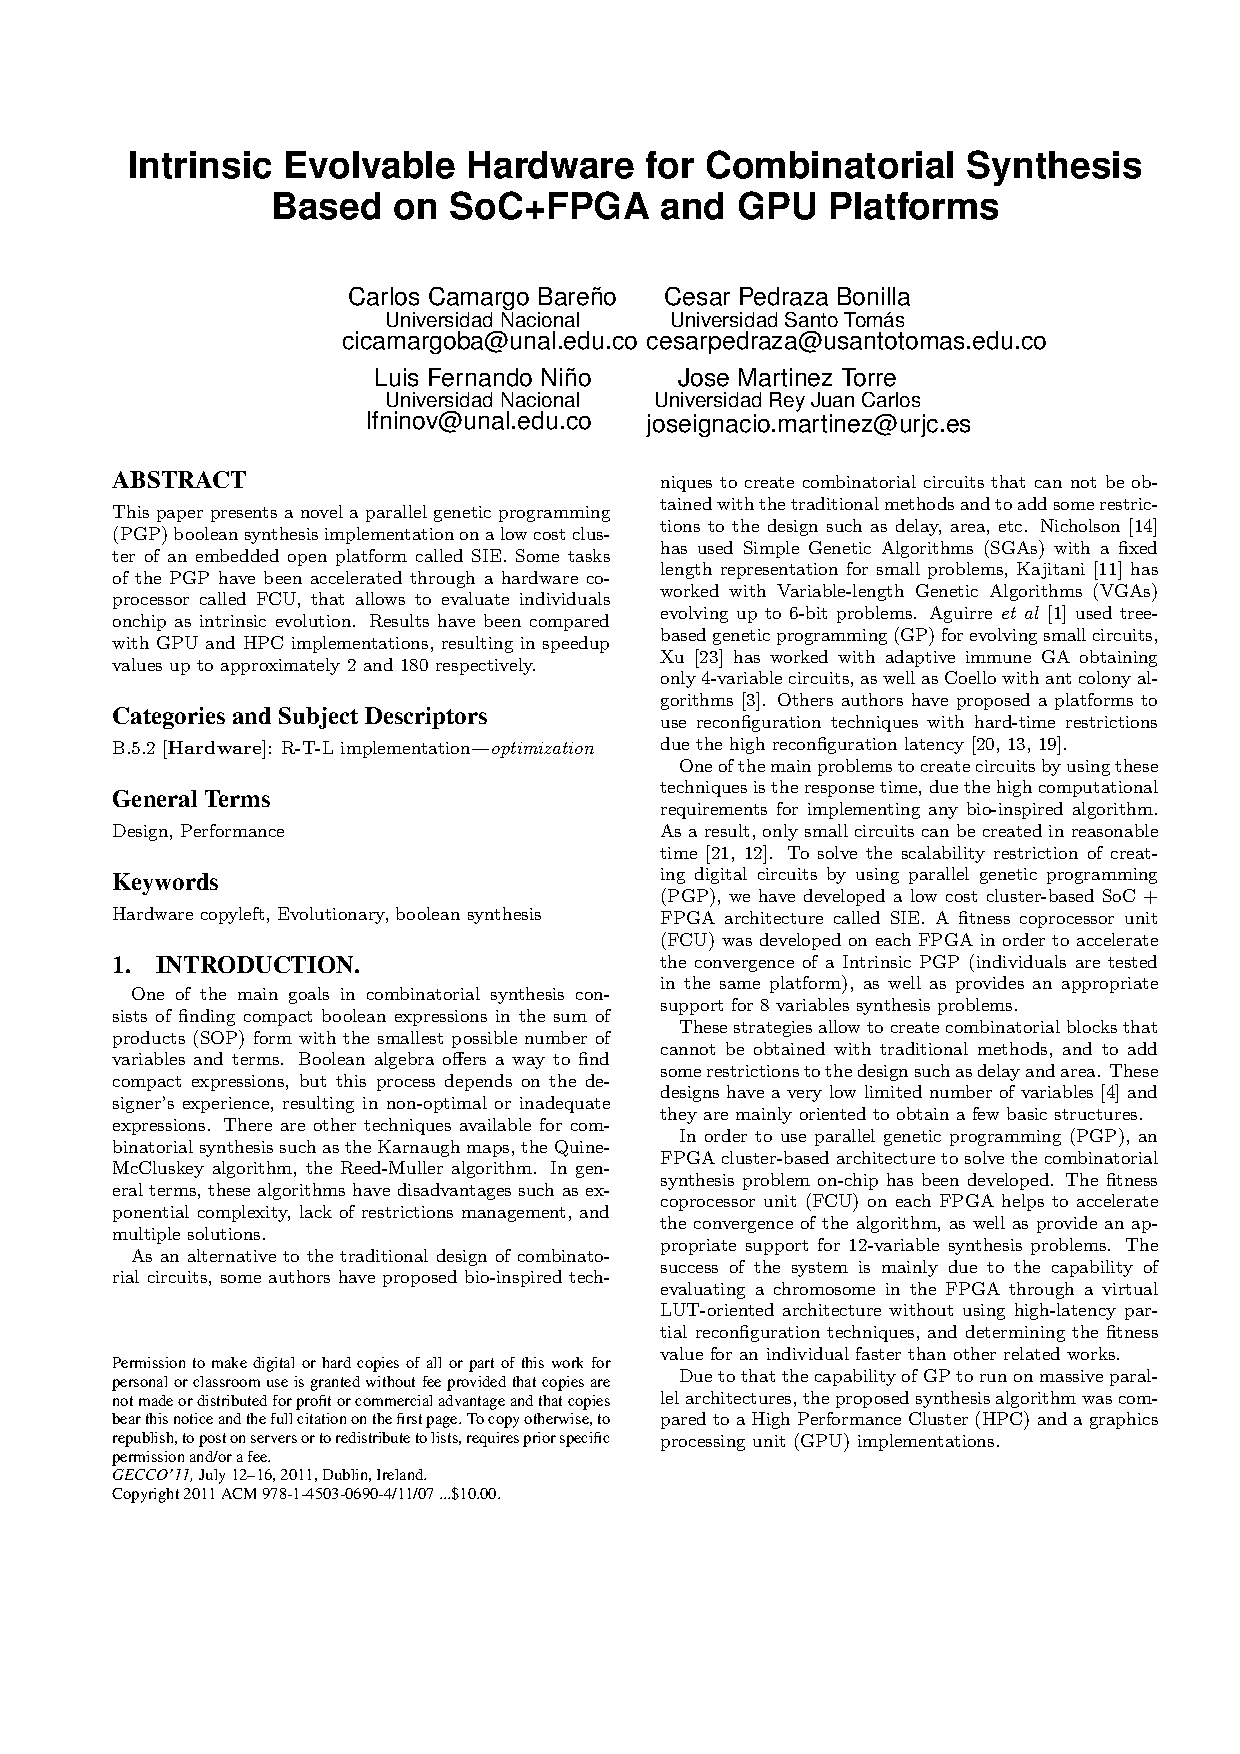
\includepdf[pages=-]{papers/gecco.pdf} 

\textbf{Low Cost Platform for Evolvable-Based Boolean Synthesis} Publicado en el 2nd IEEE \textit{Latin American Symposium on Circuits and Systems} LASCAS 2011.

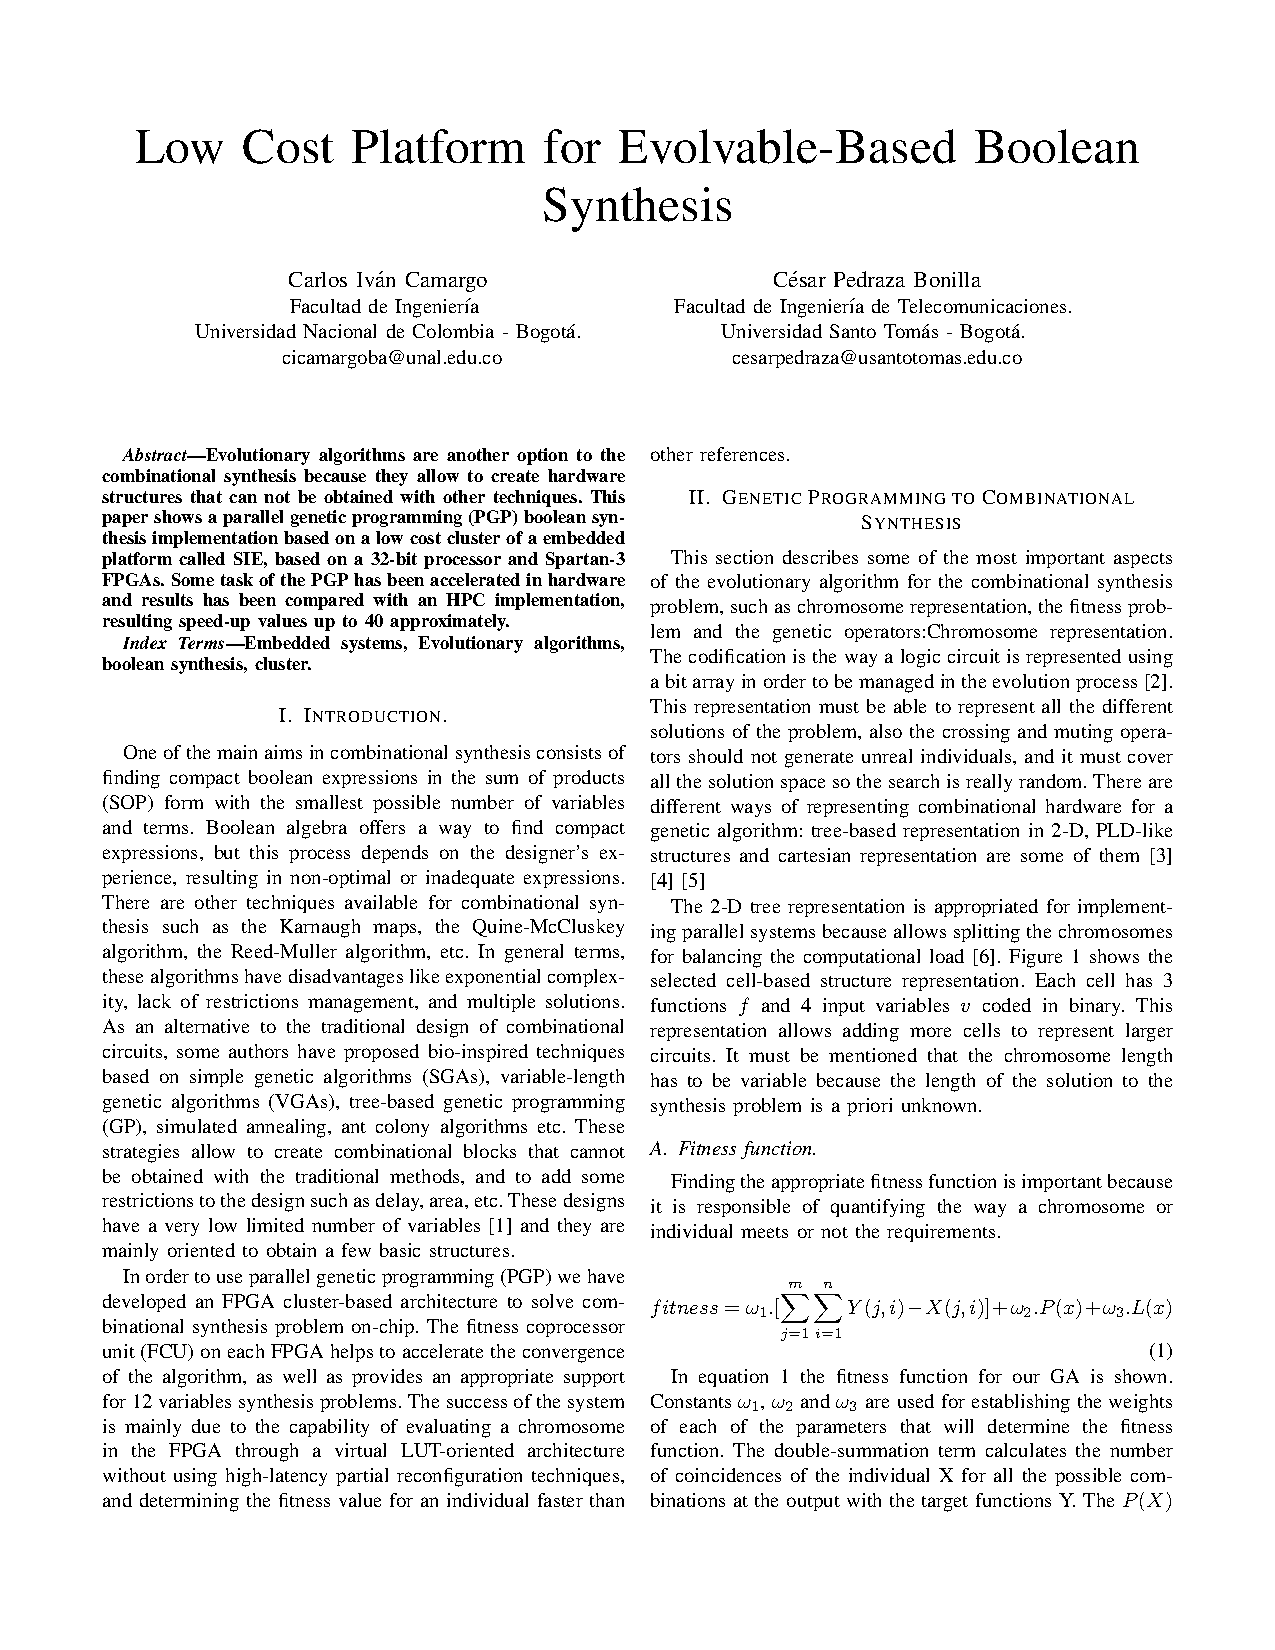
\includepdf[pages=-]{papers/ehw.pdf} 

\subsection{Aplicaciones en Rob�tica}

\textbf{CONTROL DE SISTEMAS PARALELOS INSPIRADO EN LA NATURALEZA} 3th IEEE Colombian Workshop on Circuits and Systems.
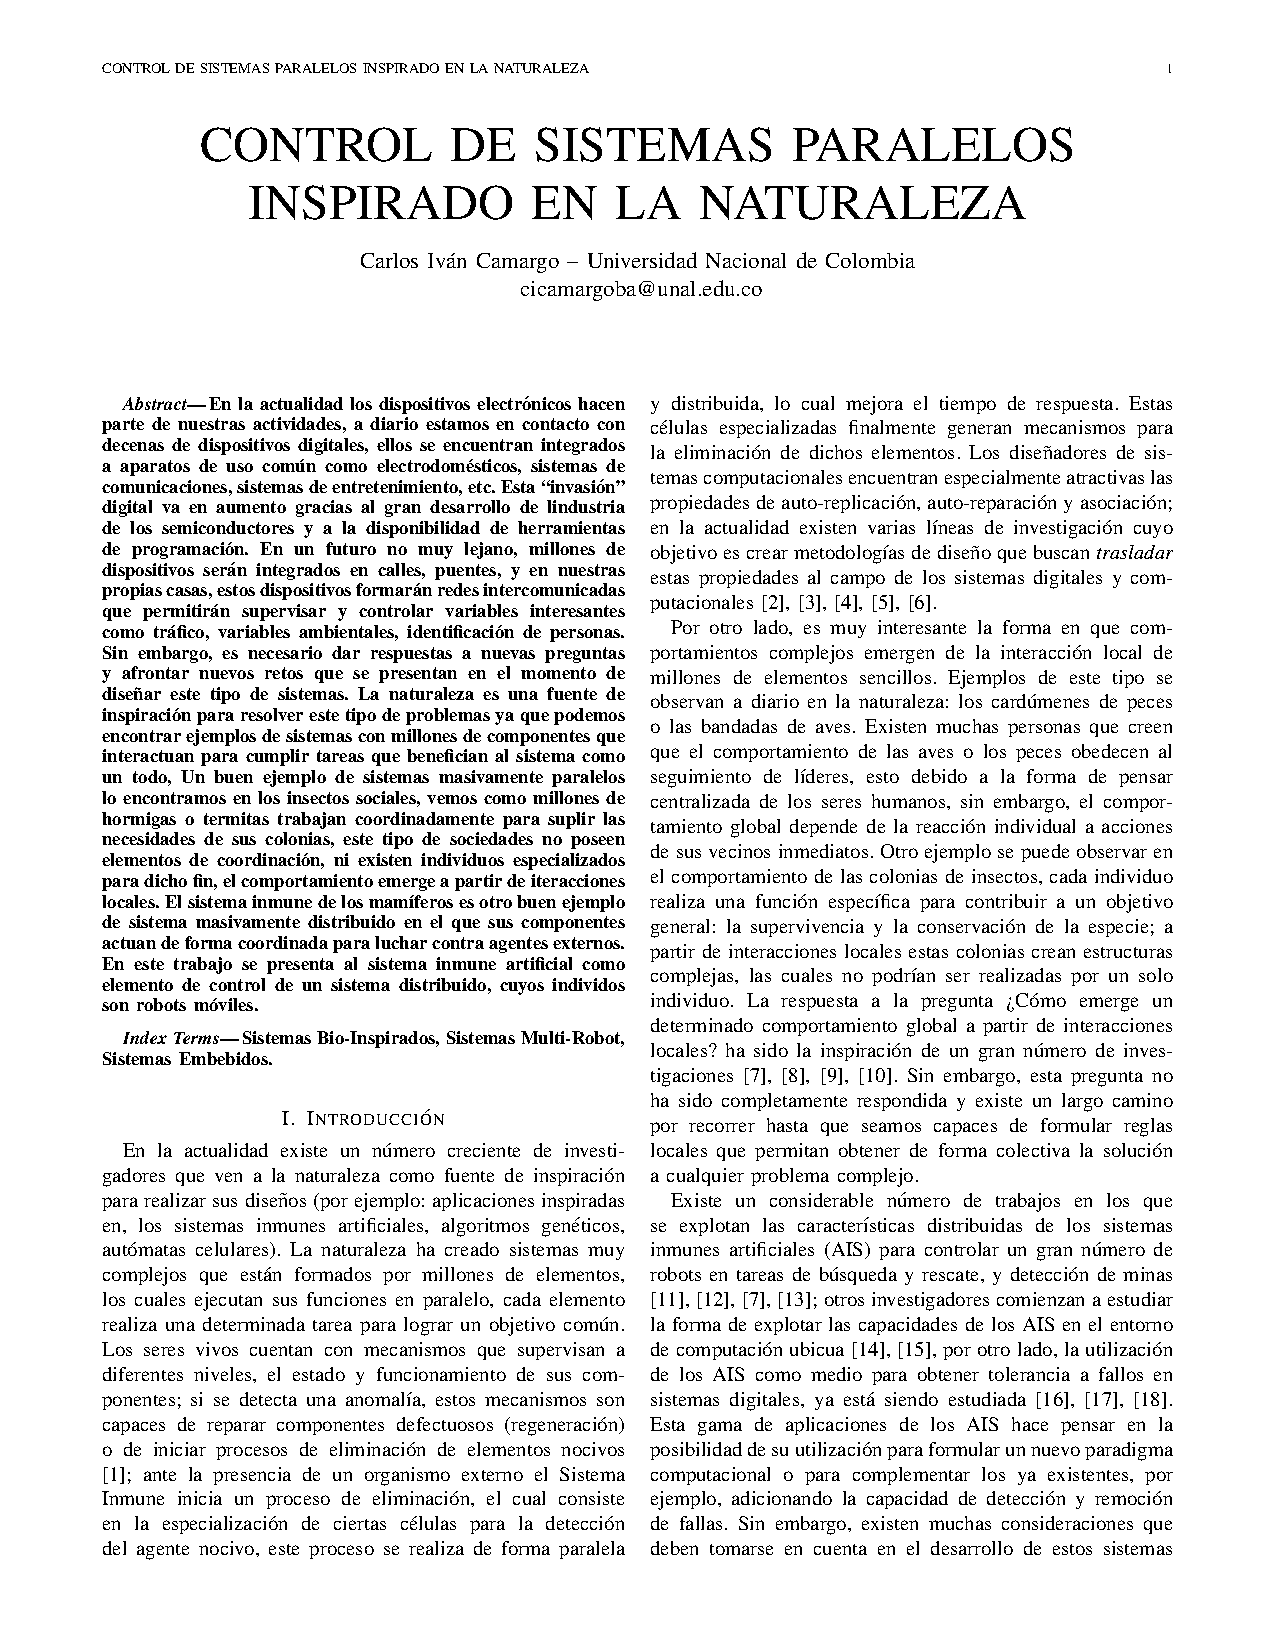
\includepdf[pages=-]{papers/CWCAS09.pdf} 

\subsection{Aplicaciones en }

\section{Sobre la Metodolog�a}

\textbf{Hardware copyleft como Herramienta para la Ense�anza de Sistemas Embebidos} Congreso Argentino de Sistemas Embebidos CASE 2011, Buenos Aires Argentina ISBN 978-987-9374-69-6
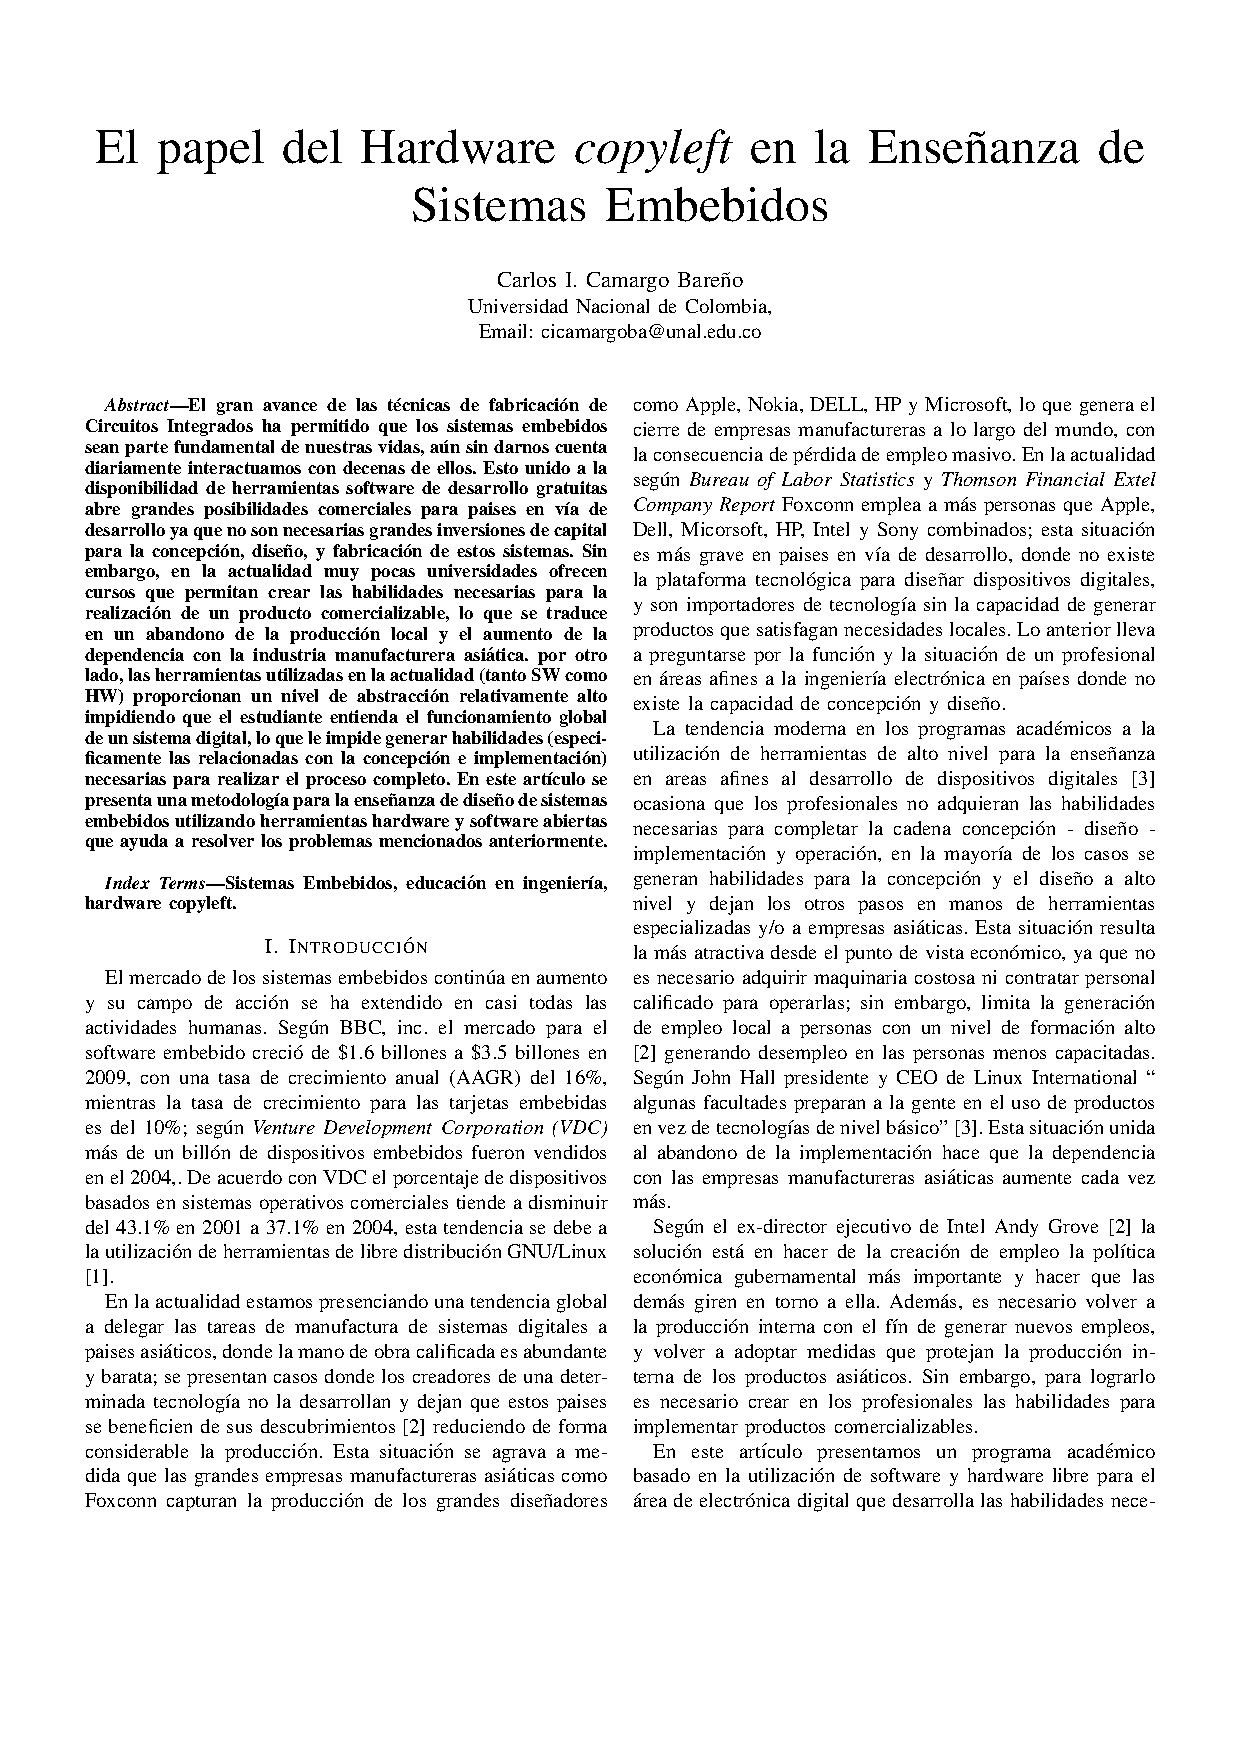
\includepdf[pages=-]{papers/CASE_2011.pdf} 

\textbf{Metodolog�a Para la Transferencia Tecnol�gica en la Industria Electr�nica Basada en Software Libre y Hardware Copyleft}. VI Congreso Internacional de la Red de Investigaci�n Y Docencia en Innovaci�n Tecnol�gica RIDIT ``Innovaci�n, Empresa Y Regi�n''.

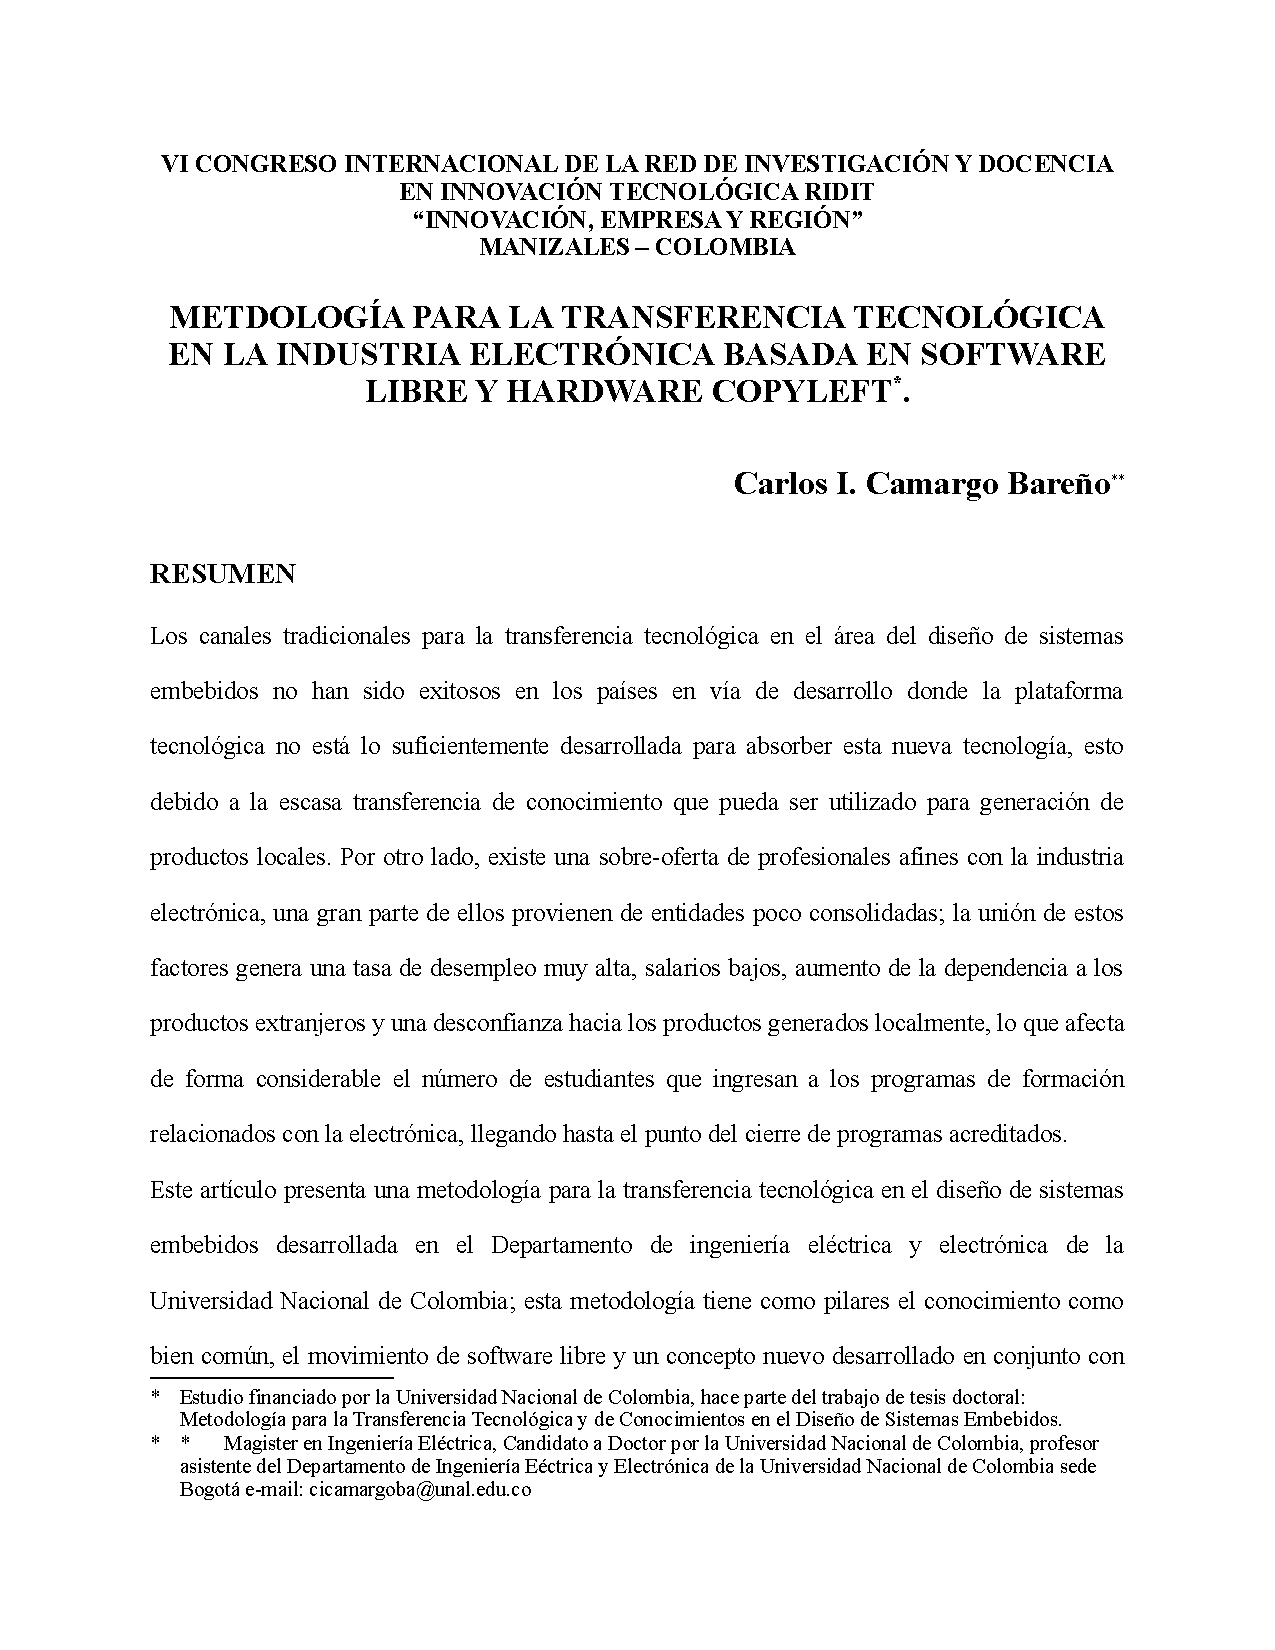
\includepdf[pages=-]{papers/RIDIT.pdf} 

\textbf{ECBOT y ECB\_AT91 Plataformas Abiertas para el Dise�o de Sistemas Embebidos y Co-Dise�o HW/SW}, VIII Jornadas de Computaci�n Reconfigurable y Aplicaciones, Madrid Espa�a.
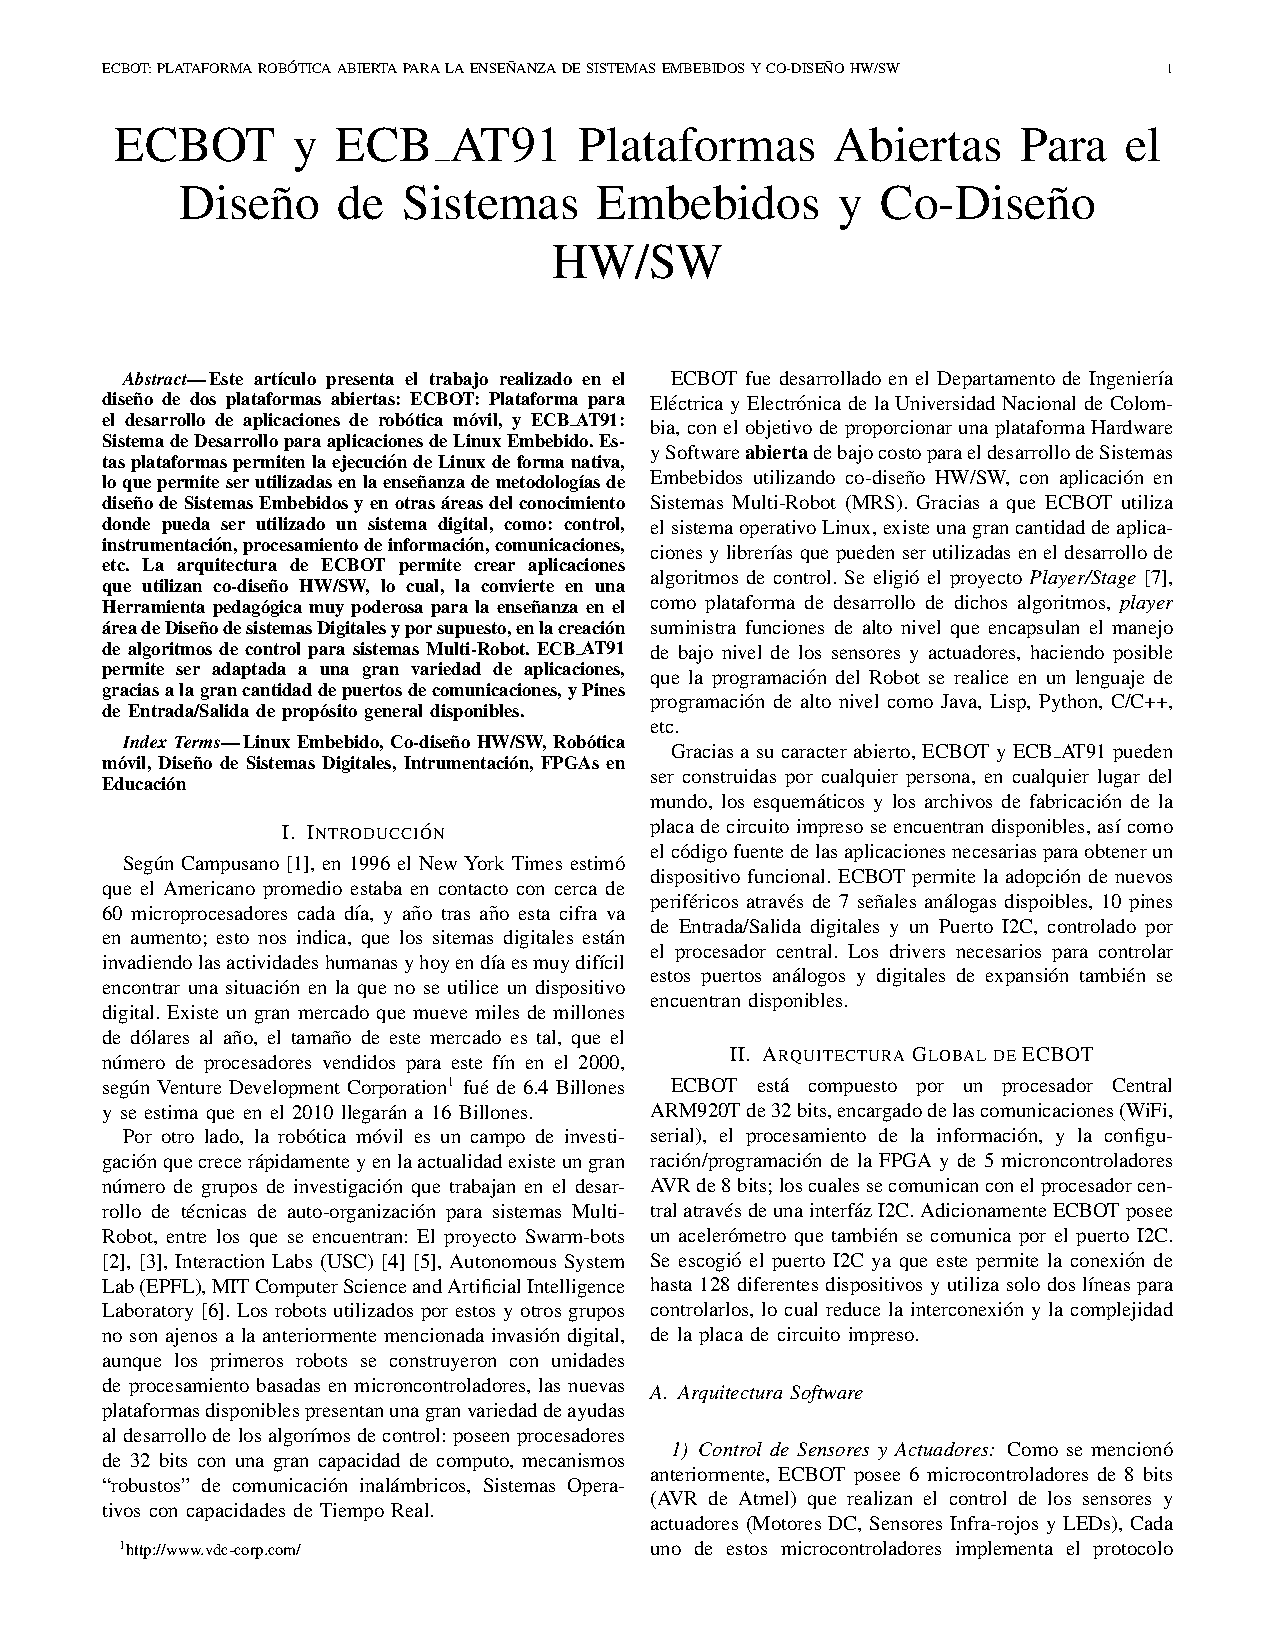
\includepdf[pages=-]{papers/JCRA_08.pdf}


\textbf{Metodolog�a Para la Transferencia Tecnol�gica en la Industria Electr�nica Basada en Software Libre y Hardware Copyleft} XVII Workshop de Iberchip 2011.
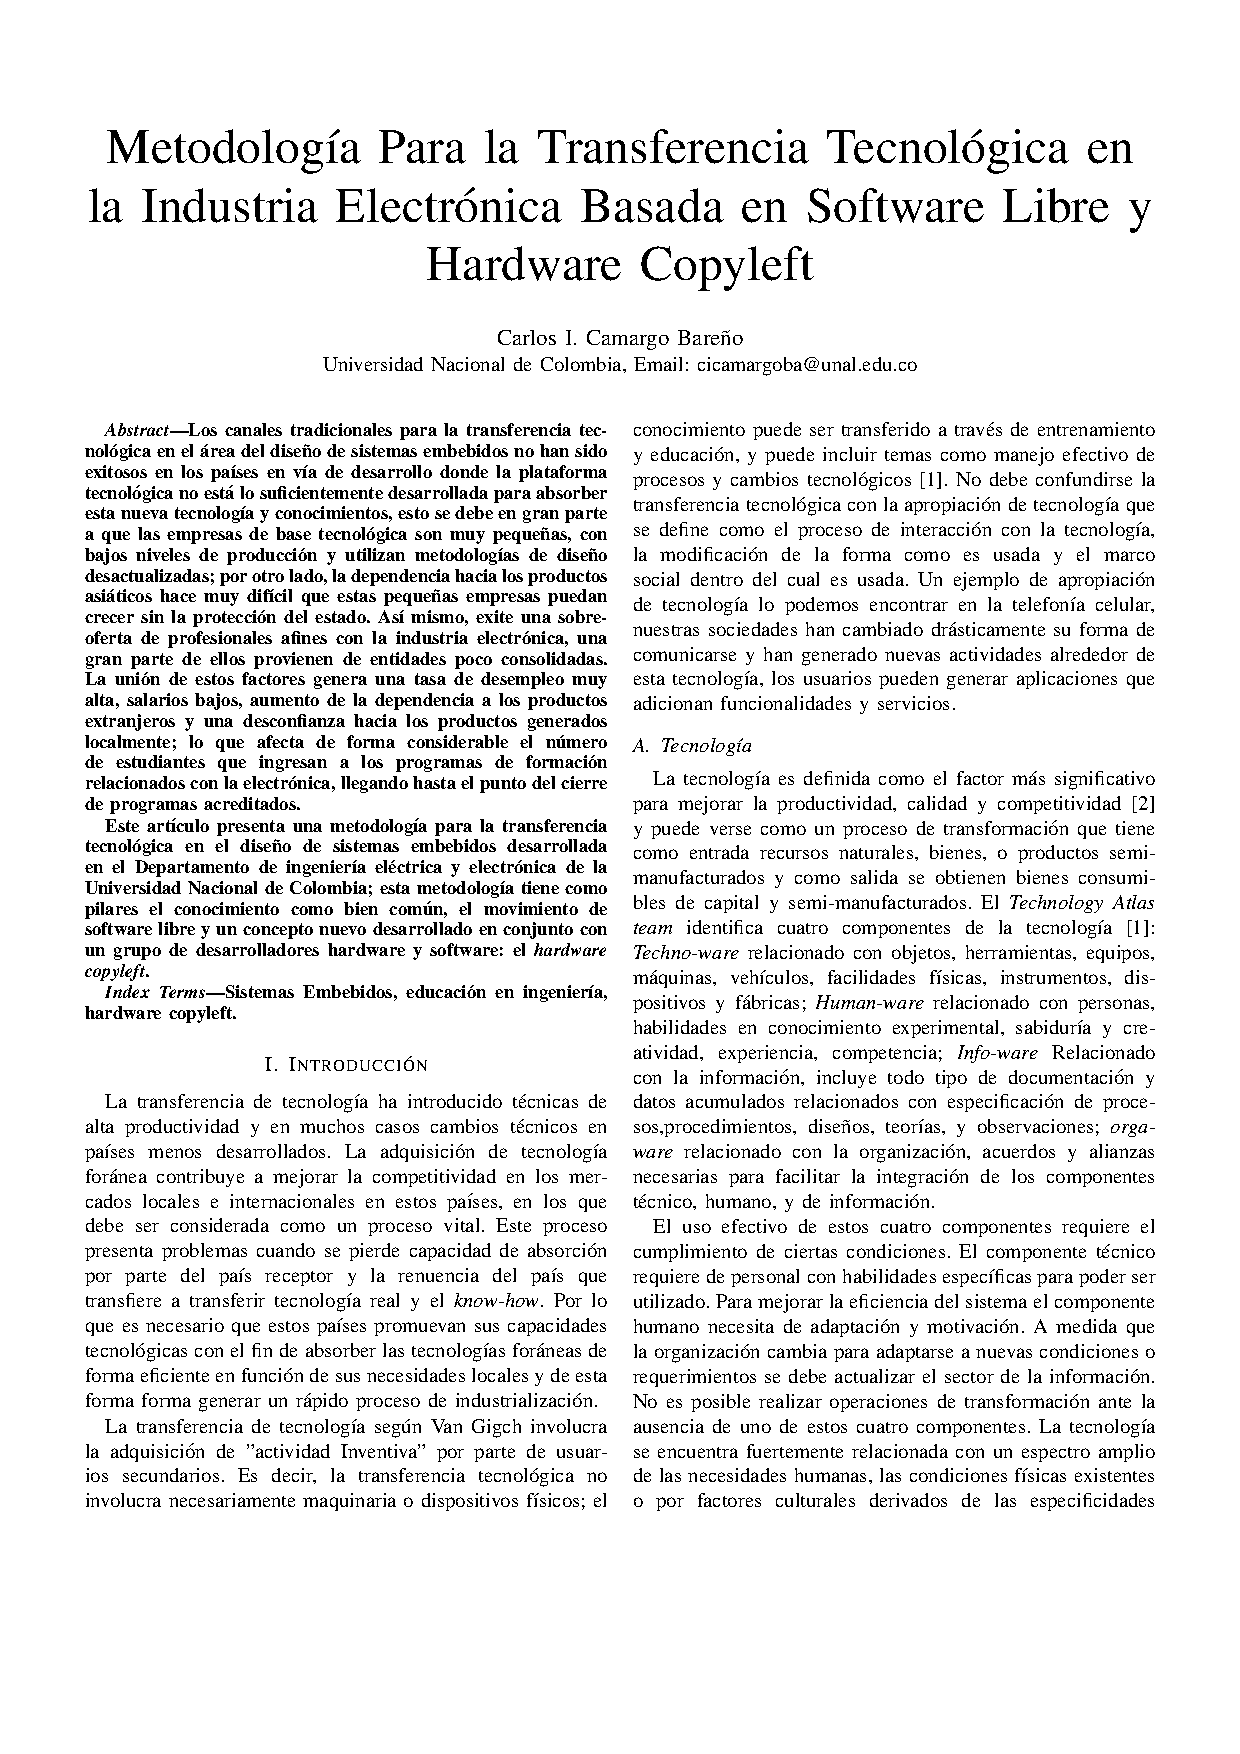
\includepdf[pages=-]{papers/Iberchip_2011_transfer.pdf} 


\textbf{SIE: Plataforma Hardware copyleft para la Ense�anza de Sistemas Digitales} XVII Workshop de Iberchip 2011.

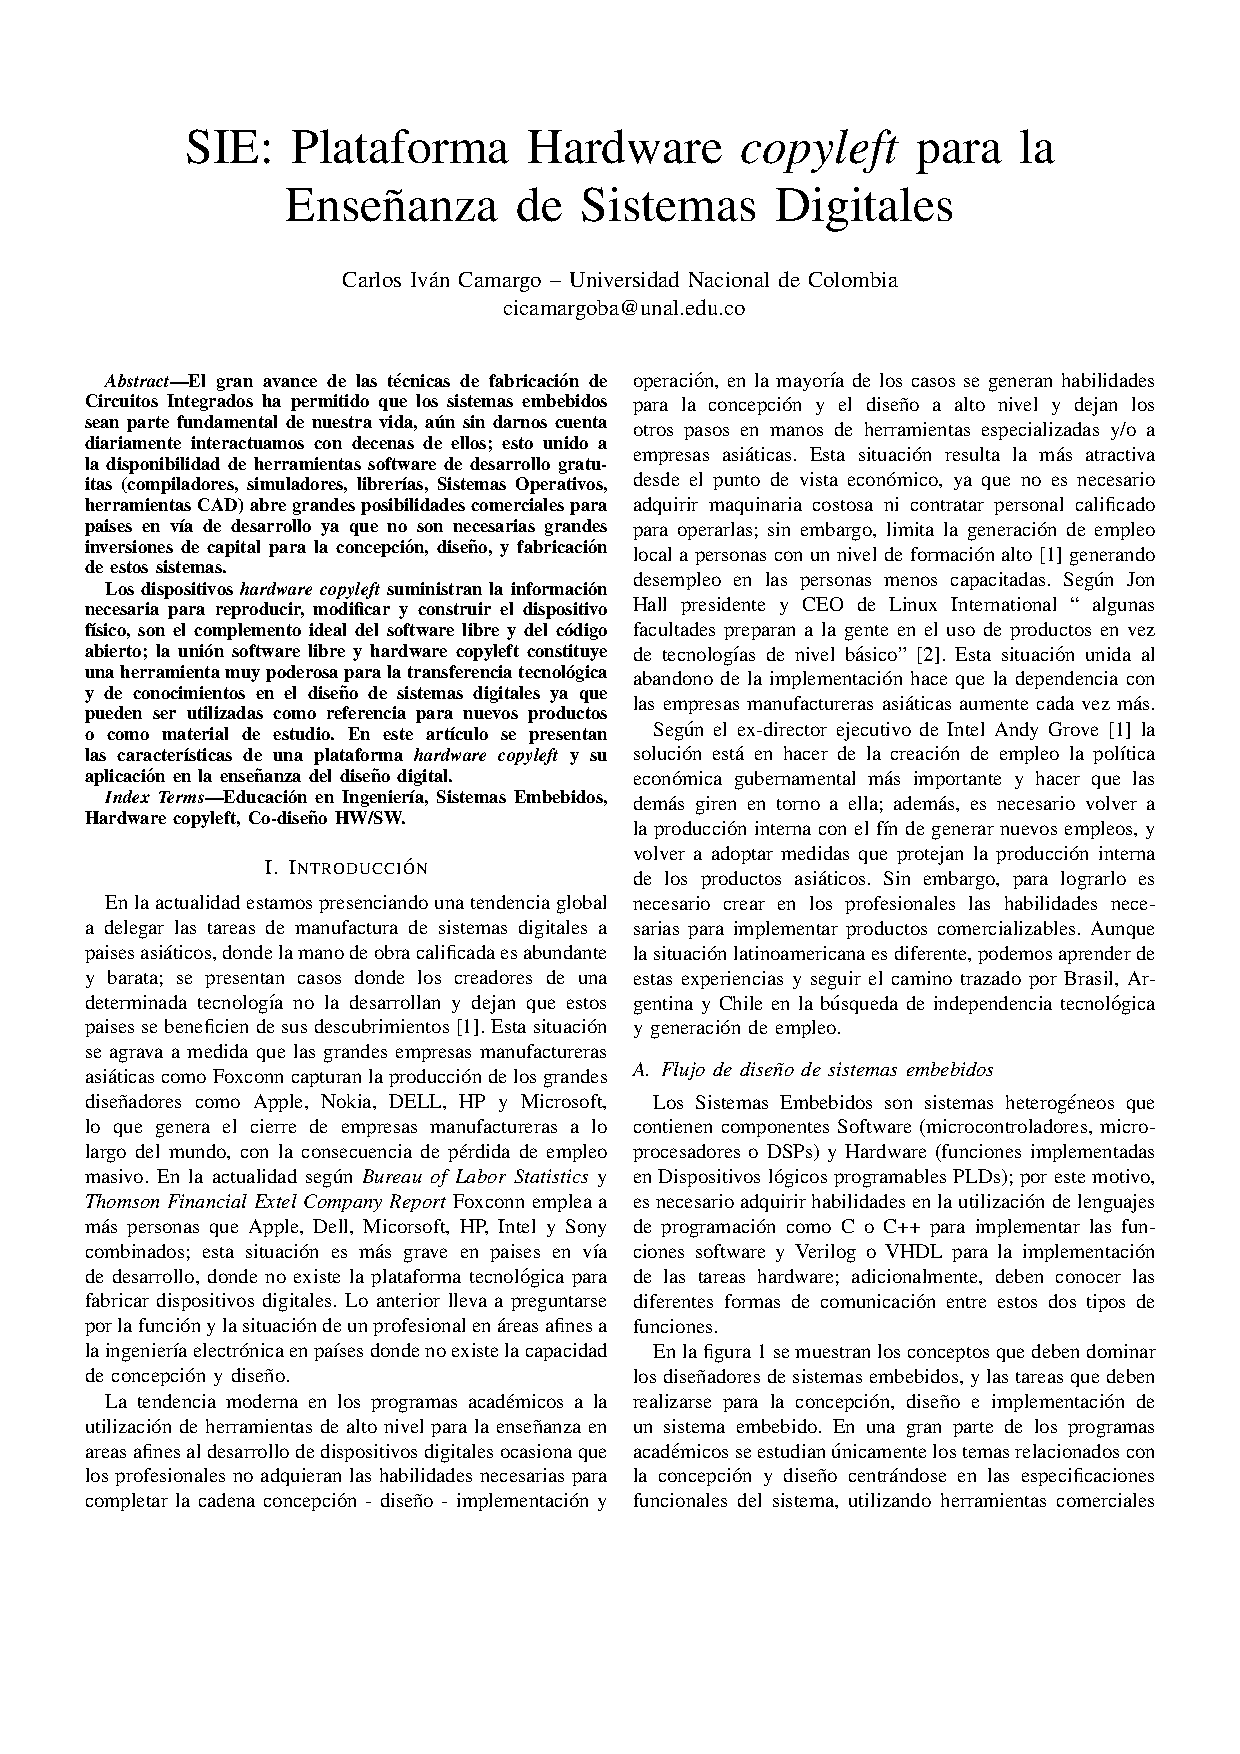
\includepdf[pages=-]{papers/Iberchip_2011_education.pdf} 


\textbf{PLATAFORMAS ABIERTAS HARDWARE/SOFTWARE PARA APLICACIONES EN ROBOTICA}, V Congreso Internacional de Ingenier�a Mec�nica y III de Ingenier�a Mecatr�nica.
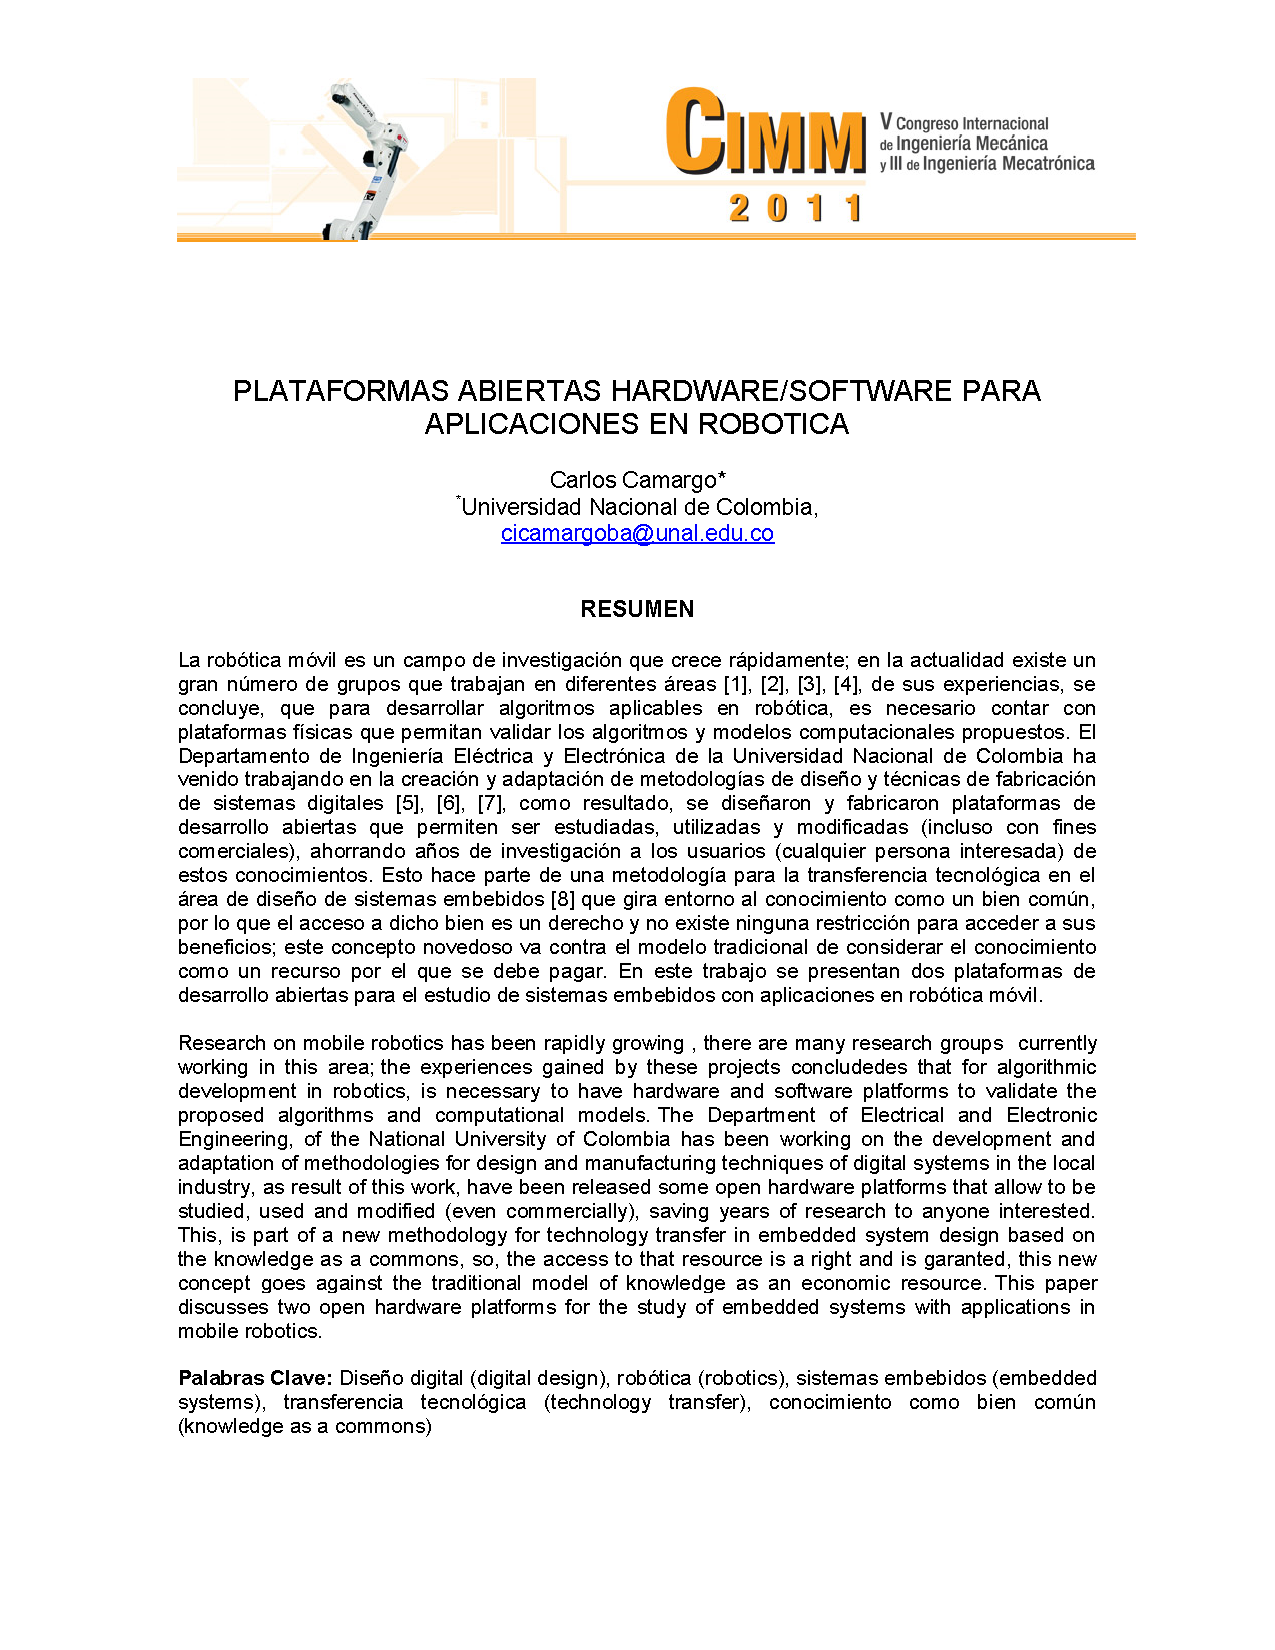
\includepdf[pages=-]{papers/CIMM_2011.pdf} 


 

% \textbf{}
% 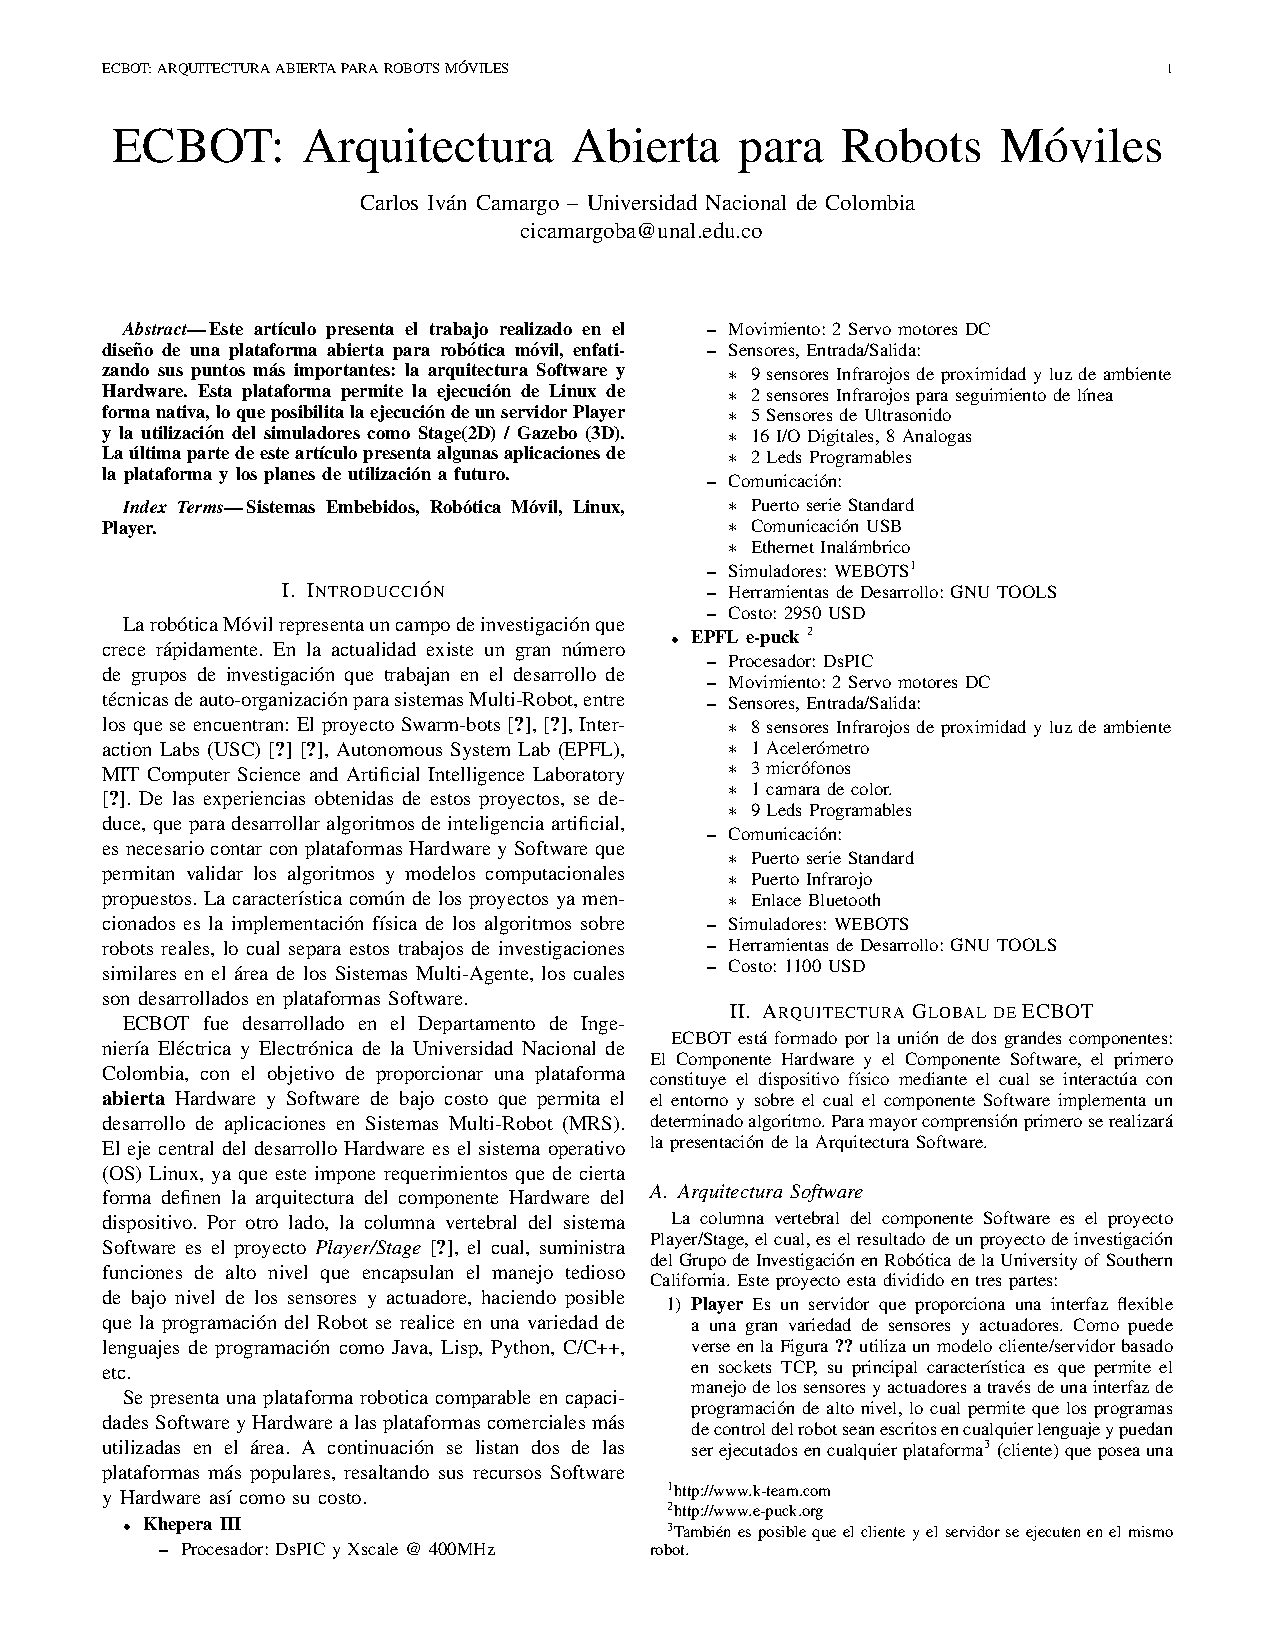
\includepdf[pages=-]{papers/CWCAS07.pdf} 
% \textbf{}
% 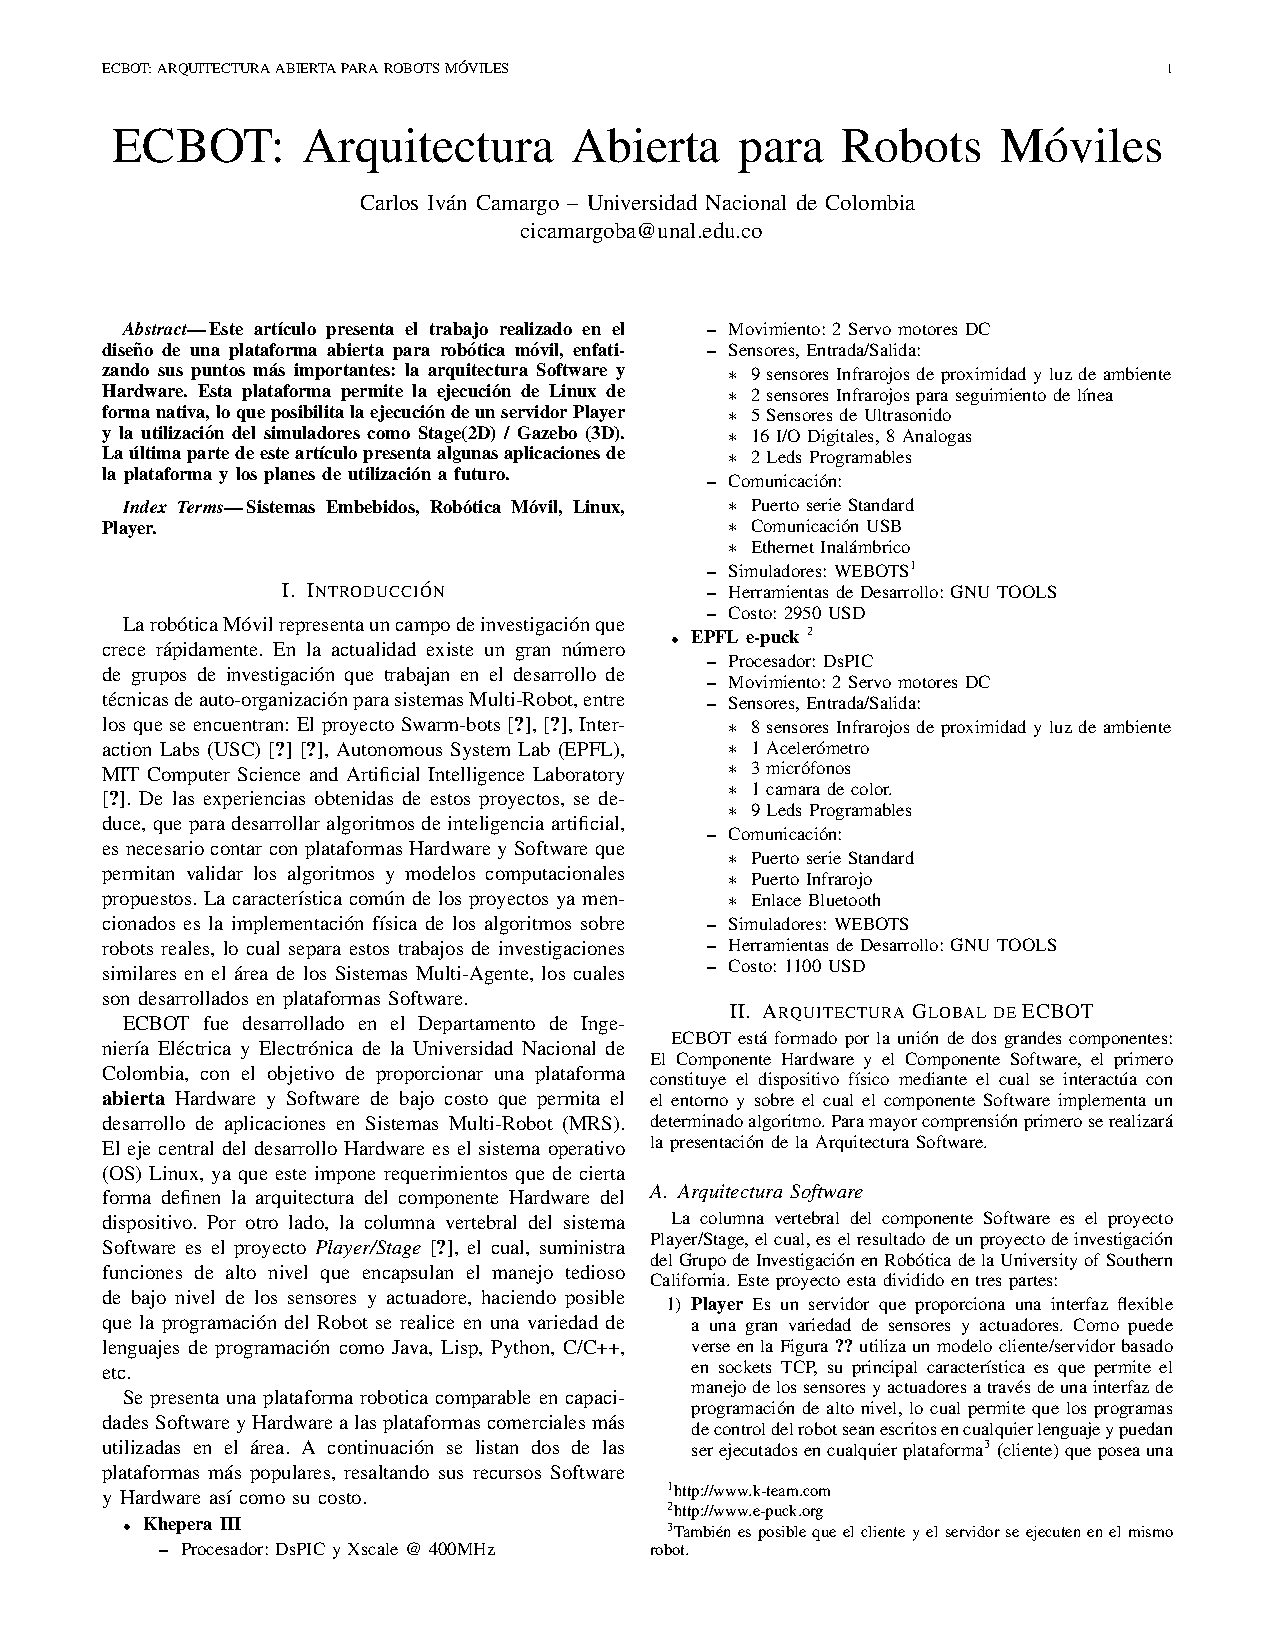
\includepdf[pages=-]{papers/CWCAS07.pdf} 
% \textbf{}
% 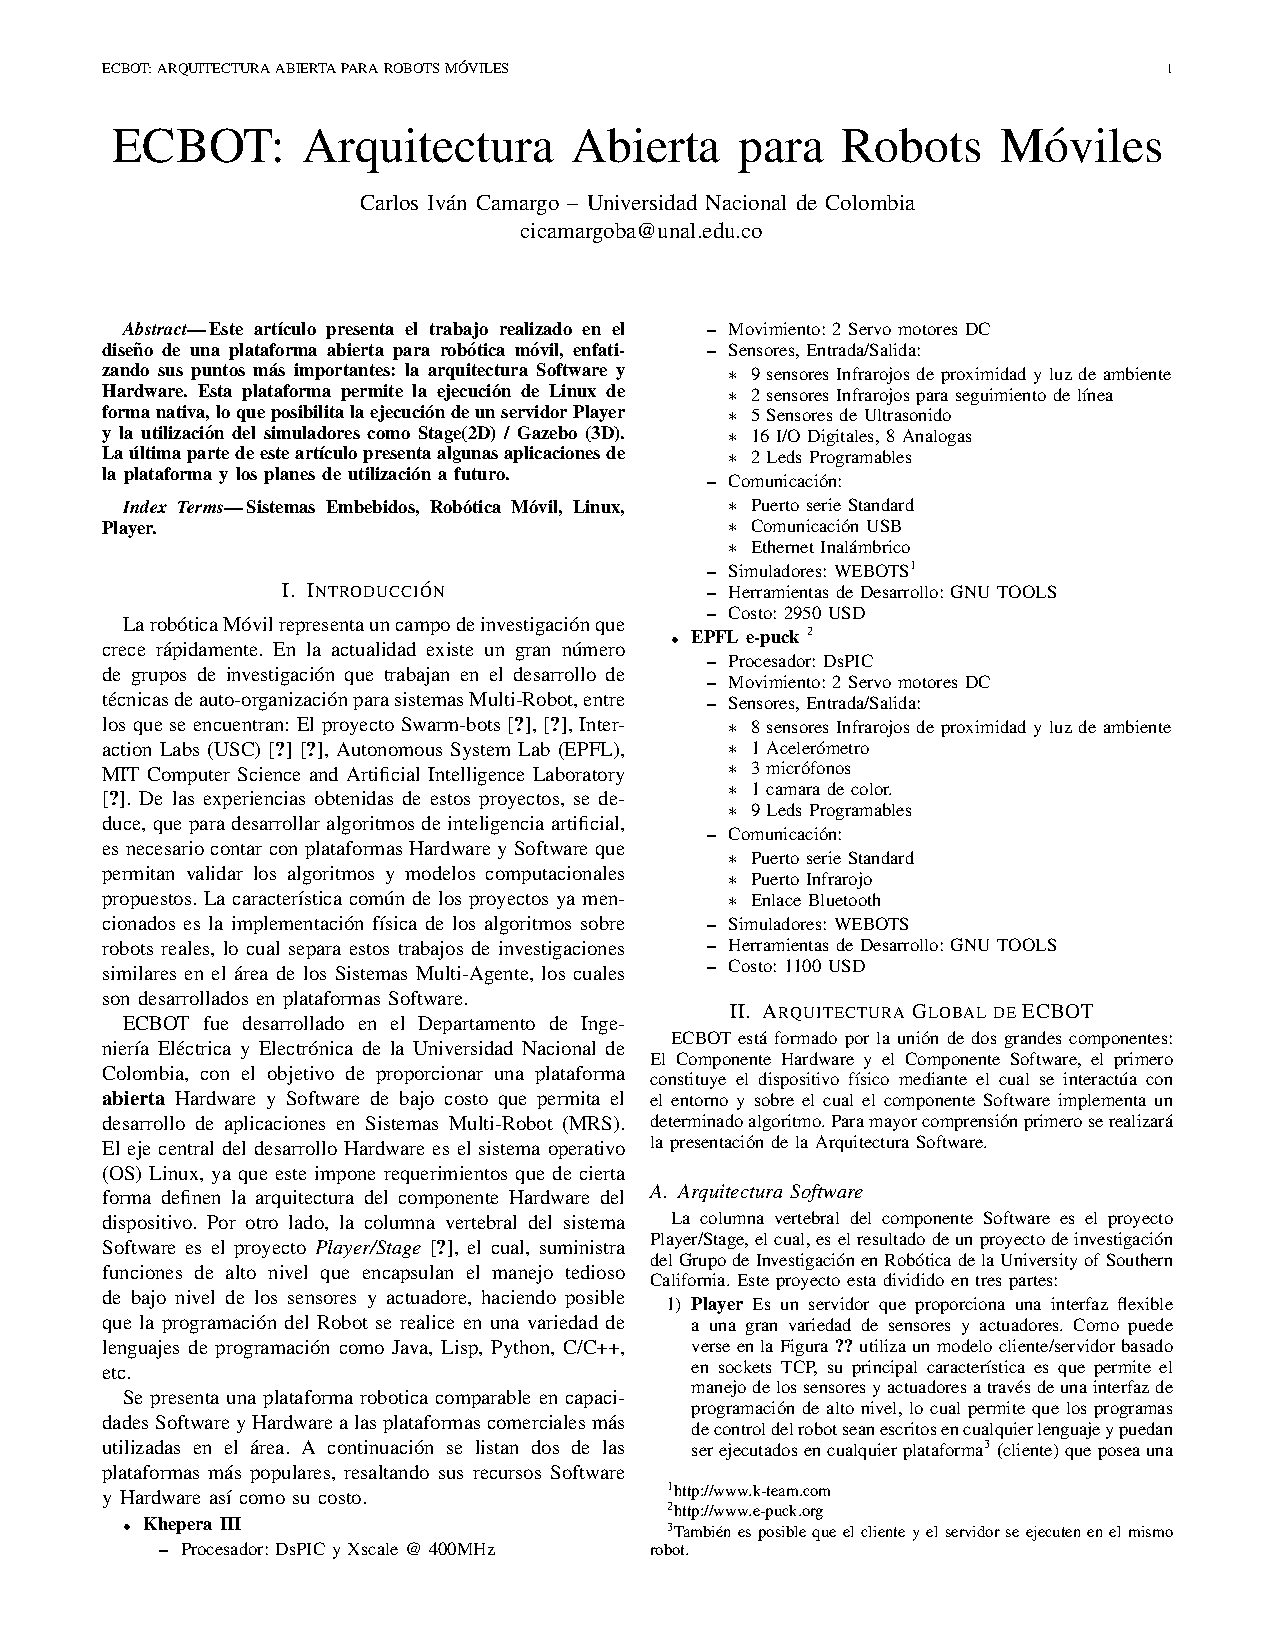
\includepdf[pages=-]{papers/CWCAS07.pdf} 
% \textbf{}
% 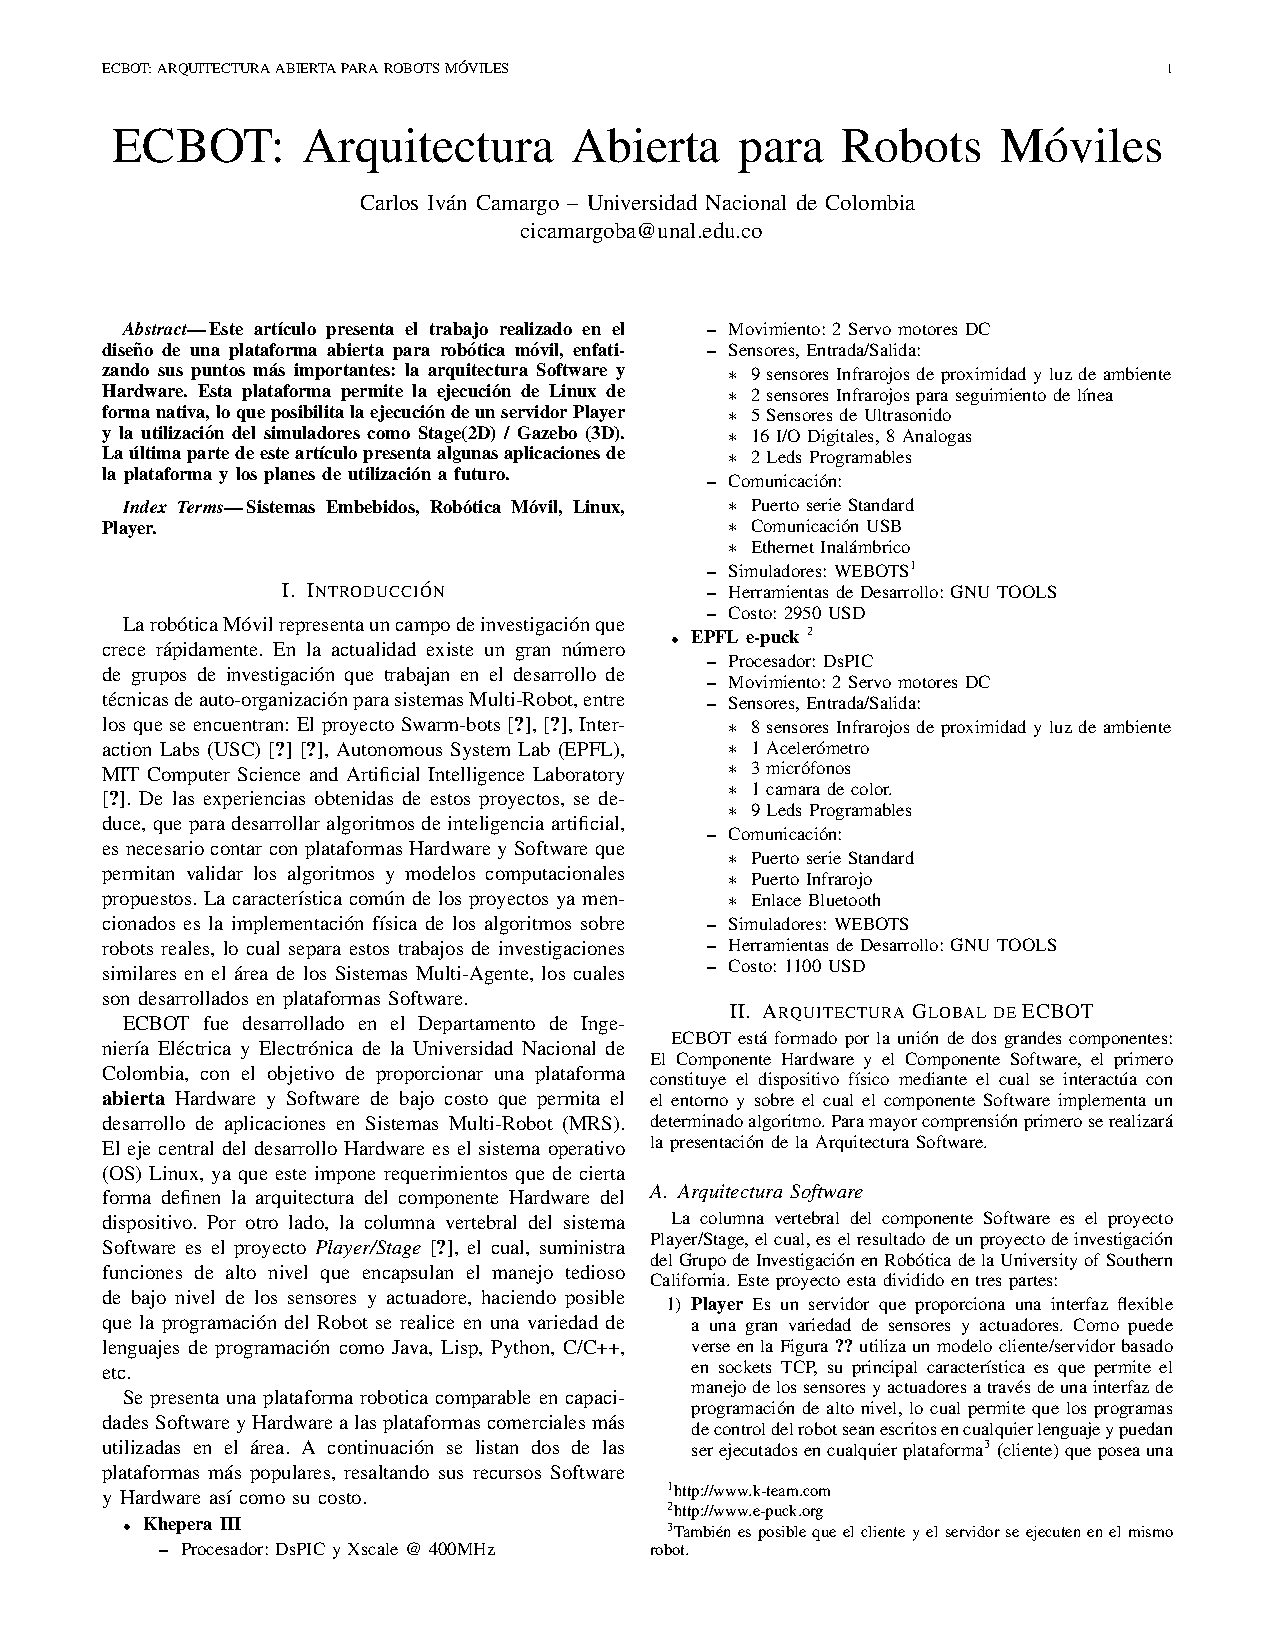
\includepdf[pages=-]{papers/CWCAS07.pdf} 
% \textbf{}
% 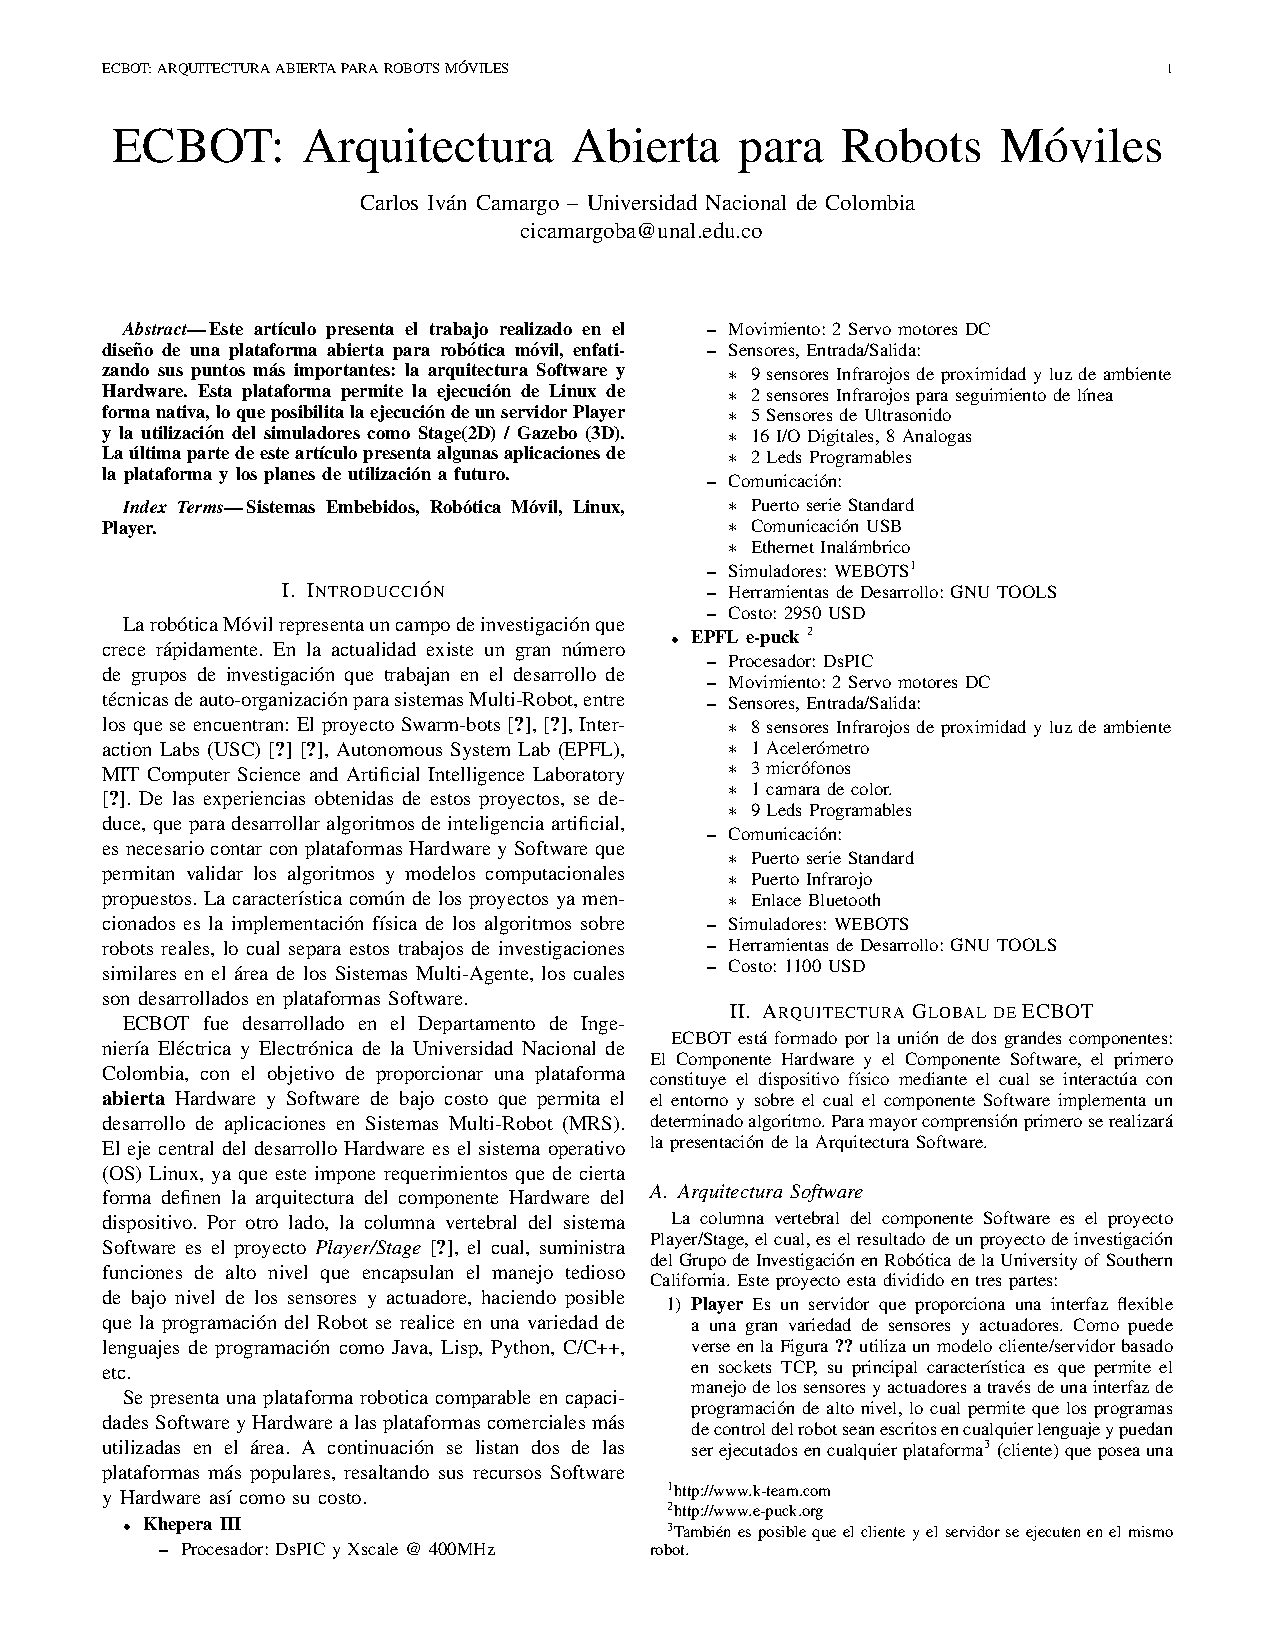
\includepdf[pages=-]{papers/CWCAS07.pdf} 




